\documentclass{article}
\def\npart {2}
\def\nterm {LMS Summer School}
\def\nyear {2021}
\def\nlecturer {Ivan Cheltsov}
\def\ncourse {Geometry of nets of conics}

\input{header}

\begin{document}
  \maketitle

\textbf{Suggested Reading} - Miles Reid, Undergrad Algebraic Geometry, contains other book recommended. Harris. Coxeter. Harsher, Schafrivich (?), Methods of Algebraic Geometry - Hodge, Ideals, Varieties and Algorithms. Complex Algebraic Surfaces by Arnaud Beauville.\\

\section{Lecture 1 - Overview}
This course is an introduction to Projective Geometry. In L3cture 1, we will consider and define the complex projective plane and lines in it, define projective transformations and their properties and finally Sylvester-Galllai Theorem.

\subsection{What is a line?}
In Algebraic Geometry we can use algebra, but it comes dry and we lose a geometric intuition.
\begin{figure}[!ht]
\centering
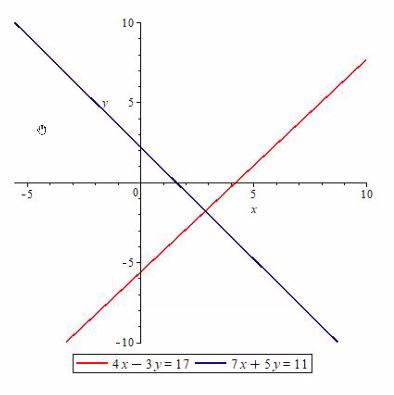
\includegraphics{./figures/L1.1}
\caption{This shows two lines intersect at one point}
\end{figure}

This picture is real, which is no good for us. Reals aren't algebraically closed, which create lots of problems and holes. If we look at the Cremona Group, theres a theorem about generators of this group, if we consider the reals, this is a really new result. Reals makes the problem too difficult and so we consider the complexes to make everything so much simpler.\\

\begin{ndefi}[Line]
  A line in $\C^2$ is a subset that is given by,
  $$ ax + by + c = 0 $$
  for some $a, b, c \in \C$ such that $(a, b) \ne (0, 0)$
\end{ndefi}

and here is a lemma,
\begin{nlemma}[]
  There is a unique line in $\C$ for rach two distinct points.
\end{nlemma}
\begin{proof}
  Trivial by linear algebra
\end{proof}

\begin{nlemma}[]
  Suppose that $L_1 \ne L_2$ then $L_1 \cap L_2$ contains at least one point.
\end{nlemma}
\begin{proof}[]
  If $a_1b_2 - a_2b_1 \ne 0$, then $L_1 \cap L_2$ consists of a point,
  % $$ \left( \frac{b_2c_2}{a} \right) $$
\end{proof}

This is what Algebraic Geometry removes.

\subparagraph{What is a plane}
For us a plane is just $\R^2$, but complex plane is also not perfect. If you don't travel over the plane that far, you are OK, but if you do, you get global problems. Take travelling the globe as an example. We can call a sphere a plane, if we wish, locally, we do, we have a plane, but global questions have a problem, the earth isn't a plane\footnote{Sorry, flat eathers}.\\


When we talk about spaces, Algebraic Geometers mean a projective plane.

\begin{ndefi}[Projective Plane]
  Let $(x, y, z) \in \C^3$ st $(x, y, z) \ne (0, 0, 0)$ and let $[x : y : z]$ be a subset of $\C^3$ such that,
  $$ (a, b, c) \in [x : y : z] \iff \begin{cases}
    a = \l x\\
    b = \l y\\
    c = \l z
  \end{cases} $$
  for some non-zero complex $\l$
\end{ndefi}

\begin{ndefi}[]
  The projective place $\P^2_\C$ is the set of all possible $[x : y : z]$
\end{ndefi}

We refer to $\P_\C^2$ as points and we can say that,
$$ [1 : 2 : 3] = [7 : 14 : 21] = [2 - i : 4 - 4i : 3 - 3i] $$
and
$$ [1 : 2 : 3] \ne [3 : 2 : 1] $$
and
$$ [0 : 0 : 1] \ne [0 : 1 : 0] $$

\begin{remark}
 There is no point $[0 : 0 : 0]$
\end{remark}

\subsection{How to live in projective plane}
Let $U_z$ be the projective plane $\pc$ consisting of points $[x : y: z]$ with $z \ne 0$,

\begin{nlemma}[]
  The map $U_z \to \C$,
  $$ [x : y: z] = \left[\frac{x}{z} : \frac{y}{z} : 1\right] \mapsto (\frac{x}{z}, \frac{y}{z}) $$
  is a bijection.
\end{nlemma}
Thus we can identify $U_z = \C^2$, we call these charts and affine charts. These are exactly manifolds are we have three affine charts.

\begin{itemize}
  \item Put $\overline x = \frac{x}{z}$ and $\overline y = \frac{y}{z}$
  \item Then we can consider $overline
  x$ and $\overline y$ coordinates on $U_z = \C62$
\end{itemize}

\begin{question}
  What is $\pc \setminus U_z$
\end{question}
\begin{itemize}
  \item The subset $\pc$ consisting of points $[ x : y : 0]$
  \item We can identify this as $\P_\C^1$
\end{itemize}
If a question isnt homogenous, it doesnt make sense to do it in $\pc$. This is the same as it is for Linear Algebra.

\begin{ndefi}[Line]
  A line in $\pc$ is the subset given by,
  $$ Ax + By + Cz = 0 $$
  for some fixed point $[A : B : C] \in \pc$
\end{ndefi}
We sometimes call $\pc$ the dual plane here. We have polynomials of degree one.

\begin{eg}
  Let $P = [5 : 0 : 2]$ and $Q = [1:-1:1]$. Then,
  $$ 2x - 3y + 5z = 0 $$
  is the unique line
\end{eg}

\begin{eg}
  Let L be give by,
  $$ x + 2y + 3z = 0 $$
  Let $L'$ be $x - y =0$, we then have $L \cap L' = [1 : -1 : 0]$
\end{eg}

\begin{nthm}[]
  There is a unique line in $\pc$ that contains $P$ and $Q$
\end{nthm}

\begin{proof}[]
  Let $L$ be a line in $\pc$ that is given by $Ax + By + Cz = 0$, then take two different lines, solve the system and by rank-nullity implies that $L$ exists and is unique
\end{proof}

\begin{nthm}[]
  The intersections $L \cap L'$ consirst of one point in $\pc$
\end{nthm}
\begin{proof}
  The same as above.
\end{proof}

It's very easy to find intersections and lines theough two points, but we can use python to do it. We can also use a determinant formula,
$$ \det \begin{pmatrix}
11 & -7 & 1\\
2 & 5 & 1\\
x & y & z
\end{pmatrix} $$

\subsection{Parallel Lines? Do they meet?}
In classical geometry, this is at infinity. We can do this in agebra,\\

Let $U_z$ be the complement of $\pc$ to the line$z= 0$. Idenity,
$$ U_z = \C $$
with coordinates $\overline x = \frac{x}{z}$ and $y = \frac{y}{z}$

\begin{itemize}
  \item Let $\overline L = 2\overline x + 3\overline y + 5 = 0$
  \item Let $\overline L = 2\overline x + 3\overline y + 7 = 0$
  \item $L \cap L' = \varnothing$
\end{itemize}

\begin{question}
  Where do $\overline L$ and $\overline L'$
\end{question}

\subsection{Projective Transformations}
If we have an equation that can be simplified using some sort of change of variables. Let $\mathbf{M} \in M_{3\times 3}$ and $\phi : \pc \to \pc$ be given by,
$$ [x : y : z] = M \mathbf{x} $$
where $\mathbf{x}$ is just the vector formed of $x$. This is called the automorphism of $\pc$, but we dont have $[0 : 0 : 0]$, this is a problem as $\phi$ may output it, if $\mathbf{x}$ is in the kernel.

\begin{question}
  When $\phi$ well defined?
\end{question}
This is when $M$ is invertible or $\det M \ne 0$

\begin{ndefi}[Projective Transformation]
  If $\det M \ne 0$ we say that $\phi$ is a projective transformation.
\end{ndefi}

\subsection{Group of transformations}

Projective transformations of $\pc$ form a group.
\begin{itemize}
  \item Let $M$ be a atric in $GL_3(\C)$
  \item Denote by $\phi_M$ the corresponding projective transformation.
\end{itemize}

\begin{question}
  When $\phi_M$ is an idenity map?
\end{question}

The map $\phi_M$ is said to be the indentity $\iff$ $M$ is a scalar.

\begin{ndefi}[]
  We call $M$ is said to be scalar if $M$ is diagonal
\end{ndefi}

\begin{ncor}
   Let $G$  be a subgroup in $GL_3(\C)$ consistong of scalar matrices. The group of projective transformations of $\pc$ is isomorphic to,
   $$ PGL_3(\C) = GL_3(\C)\/G $$
\end{ncor}

We can look at mobius transformations, but for our plane. If you have four points in the plane, such that no three points are not collinear. Then there is a projective plane such that $\pc \to \pc$ such that,
$$ [1:0:0], [0:1:0], [0:0:1], [1:1:1] $$
so we let, $P_1 = [a_{11} : a_{12} : a_{13}]$ and $P_2 = [a_{21} : a_{22} : a_{23}]$ and $P_3 = [a_{31} : a_{32} : a_{33}]$ and then do $\phi$ on them and then it will map the basic points to ir points and so do the inverse. Let $\psi$ be $\phi$ and then apply it and then forma projective transformation and done.

\subsection{Sylvester - Gallai Problem}
\begin{problem}
  Let $\Sigma$ be the finite subset in $\R^2$. show that either $\Sigma$ is contained in one line, or there is a line containing exactly two points in $\Sigma$.
\end{problem}
\begin{itemize}
  \item This problem was proposed by Sylvester in 1893
  \item It was solved by Gallai in 1944
  \item A simpler proof was given by Kelly in 1948
\end{itemize}

Sylvester was not just a Geometry, he was interested in Algebra aswell, he worked with Complexes and he knew the problem was wrong. He knew a very simpler counter example.\\

\subsection{Hesse Configurations}


\begin{itemize}
  \item Nine points were the counterexample
  \item There are 12 lines passing through 2 points among them
  \item Each such line contain 3 points among nine.
\end{itemize}

\begin{figure}[!ht]
\centering
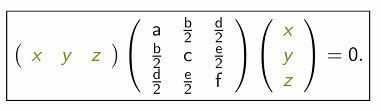
\includegraphics{./figures/L2.1}
\end{figure}

\begin{itemize}
  \item Let $\F$ be a field
  \item Let $\Sigma$ be a finite subset in $\P_\F^2$
\end{itemize}

Suppose that the subset $\Sigma$ is not contained in one line,

\begin{nlemma}[]
  There exists a line in $\P_\F^2$ contaning exactly two points in $\Sigma$,
  \begin{itemize}
    \item where $|\Sigma| \le 6$
    \item where $|\Sigma| = 7$ and $2 \ne 0$ in $\F$
    \item where $|\Sigma| = 8$
  \end{itemize}
\end{nlemma}

\begin{nthm}[]
  Suppose $|\Sigma| = 9$ and $\F=\C$. If there exists no line containing exactly two points of the set
\end{nthm}

\section{Lecture 2 - Conics}
In this lecture we will cover,
\begin{itemize}
  \item Conics in the complex projective Plane
  \item Classifications of conics up to projective Transformations
  \item Intersections of conics and lines in $\pc$
  \item Intersections of two conics (Bezout Theorem in disguize)
\end{itemize}

\subsection{Conics in the complex projective plane.}

\begin{ndefi}[Conic]
  A conic in $\pc$ is a subset that is given by,
  $$ ax^2 + bxy + cy^2 + dxz + eyz + fz^2 = 0 $$
  for $a, b, c, d, e, f \in \C$ such that $(a, b, c, d, e, f) \ne (0, 0, 0,0,0,0)$
\end{ndefi}

The right way to think about this, is a curve. This was traditionally defined as a section as a conic in the cartesian plane.

\begin{ndefi}[Irriducible]
  The conic is said to be irreducible if
  $$ ax^2 + bxy + cy^2 + dxz + eyz + fz^2 = 0 $$
  is irreducible, Otherwise the conic is reducible, i.e. can be factored as two linear terms or lines.
\end{ndefi}

A conic is the union of two lines. The topology of an irreducible conic is just a sphere.\\

Let $\mathcal{C}$ be a conic in $\pc$. Then $\mathcal{C}$ that is given by,
$$ ax^2 + bxy + cy^2 + dxz + eyz + fz^2 = 0 $$
and we can rewrite the equation in matrix form,
\begin{figure}[!ht]
\centering
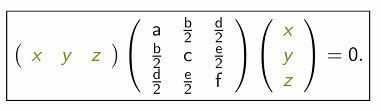
\includegraphics{./figures/L2.1}
\end{figure}

and this is just the Hessian of the conic.
 \begin{nlemma}[]
   The conic $\mathcal{C}$ is irreducible if and only if $\det M \ne 0$.
 \end{nlemma}

\begin{eg}
  The conic $xy - z^2 = 0$ is irreducible.
\end{eg}

\subsection{Five Points make a conic}
Let $P_i \in \pc$ for $1\le i \le 5$. Suppose no four points is collinear.

\begin{nthm}[]
  There is a unique conic in $\pc$ that contains these points
\end{nthm}

\begin{proof}[]
  Write down the coordinates of the points, every two points can be cooked up a line, then check three points. Find complex numbers such that,
  \begin{figure}[!ht]
  \centering
  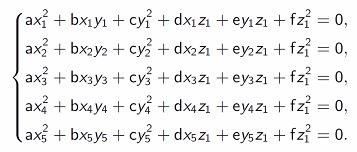
\includegraphics{./figures/L2.2}
  \caption{}
  \end{figure}
These are linear, apply rank-nullity and then it's dimension is not zero. Find null space, so there is at least one conic. Next proof that the rank is not larger than five, or is exactly five.
\end{proof}

\subsubsection{How to find a conic?}
It would be time consuming by hand, so do it with Python. We can plot the real part of the curve as just curves.

\subsubsection{Intersection of line and a conic}
Let $L$ be a line in $\pc$. Let $C$ be an irreducible conic in $\pc$

\begin{nlemma}[]
  The intersection of $L \cap C$ consists of 2 points.
\end{nlemma}

\begin{proof}[]
  The $L$ is given by,
  $$ \a x + \b y + \g z = 0 $$
  for $\a, \b, \g \in \C$ such that they are non-zero. The conic $C$ is given by,
  $$ ax^2 + bxy + cy^2 + dxz + eyz + fz^2 = 0 $$
  for $a, b, c, d, e, f \in \C$ such that ... . Then $L \cup C$ is,
  $$ \begin{cases}
    \a x + \b y + \g z = 0 \\
    ax^2 + bxy + cy^2 + dxz + eyz + fz^2 = 0
  \end{cases} $$
  which then has solutions, which are 2 as we have a quadratic.
\end{proof}

If we consider, an example.
\begin{eg}
  $L : 2x + 7y - 5z = 0$ and $C : 2x^2 -3xy + 7y^2 - 5xz + 11yz - 8z^2$. Firstly we check at infinity. The intersection of $L_z \cap L \cap \mathcal{C}$ and see this is empty, then look at non-infinity, by letting $z = 1$, and substitute and get quadratic equations and get two numbers. If discriminant is negative, this isn't a problem as we are algebraically closed.
\end{eg}

Let $L$ be a line in $\pc$, and let $\mathcal{C}$ be irreducible in $\pc$.

\begin{question}
  When $|L \cap \mathcal{C}| = 1$?
\end{question}

If we consider finite fields, our pictures are intuitive, but we can still study tangents. We may assume $[0:0:1] \in L \cap \mathcal{C}$. Then $\mathcal{C}$ is given by,
$$ \mathbf{a}x^2 + \mathbf{b}xy + \mathbf{c}y^2 + \mathbf{d}xz + \mathbf{e}yz = 0 $$
for some $[\mathbf{a} : \mathbf{b} : \mathbf{c} : \mathbf{d}] \in \P_\C^4$.\\
we may assume that $L$ is given by $x=0$. Then,
$$ L\cap \mathcal{C} = [0 : 0 : 1] \cup [0 : \mathbf{e} : -\mathbf{c}] $$
and so we have $|L \cap \mathcal{C}| 0 \iff \mathbf{e} = 0$.\\

\begin{itemize}
  \item Let $U_z$ be the complement in $\pc$ to the line $z = 0$
  \item Identify $U_z = \C^2$ with coordinates $\overline x = \frac{x}{z}$ and $\overline y = \frac{y}{z}$
\end{itemize}
Then $U_z \cap \mathcal{C}$ is given by $\mathbf{a}\overline x^2$

\begin{figure}[!ht]
\centering
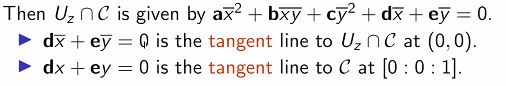
\includegraphics{./figures/L2.3}
\end{figure}

Then $|L \cap \mathcal{C}| = 1 \iff$ $L$ is tangent to $\mathcal{C}$ at point $L \cap \mathcal{C}$

\subsection{Conics and projective transformations}
Let $\mathcal{C}$ be a conic,
\begin{nthm}[]
  There is projective transformations $\phi$ such that $\phi(\mathcal{C})$ is given by,
  \begin{enumerate}
    \item either $xy = z^2$ (irreducible smooth conic)
    \item $xy = 0$ (a union of two lines in $\pc$)
    \item $x^2 = 0$ (a line in $\pc$ taken with multiplicity 2)
  \end{enumerate}
\end{nthm}
The proof could use Grahm Schmitz Orthogonalisation.\footnote{This is course is made acessible ;)} We can instead do group thory by studing an 8 dimensional group. We will then quotient this with three orbit (one normal, two special (unstable)).

\begin{itemize}
  \item Pick a point in $\mathcal{C}$ and map it to $[0 : 0 : 1]$. This {\color{blue} kills }$f$.
  \item Map the tangent line $dx + ey = 0$ to $x = 0$. This {\color{orange} kills }$e$.
  \item Map the line $z = 0$ to the line,
  $$ z + \a y + \b z $$
  for appropriate $\a, \b$ to {\color{green} kills} $a$ and $b$
  \item Scale $x, y$ and $z$ to get $b = 1$ and $c = - 1$
\end{itemize}
This gives a projective Classification, i.e. the conic is just
$$ xy = z^2 $$

\subsection{Intersecting Two Conics}

\begin{nthm}[]
  The intresection of $\mathcal{C} \cap \mathcal{C}'$ consists one one, two or three or four points.
\end{nthm}

\begin{proof}[]
  We can use Classification theorem, so just go to $xy = z^2$.
  \begin{itemize}
    \item Let $L$ be the line $y = 0$. Then $L \cap \mathcal{C} \cap \mathcal{C}' \subset [1 : 0 : 0]$
    \item One has $L \cap \mathcal{C} \cap \mathcal{C}' = [1 : 0 : 0] \iff a = 0 $
    \item Let $U$
  \end{itemize}
  \begin{figure}[!ht]
  \centering
  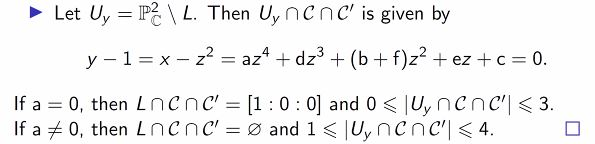
\includegraphics{./figures/L2.4}
  \caption{}
  \end{figure}
\end{proof}

Here are some examples

\section{Lecture 3 - Cubics}
In this lecture,
\begin{itemize}
  \item Cubics curves in the complex projective plane
  \item Each smooth cubic curves in $\pc$ has 9 infection points
  \item Classification of cubics up to projective transformations
  \item Legendre, Weirstrass and Hesse forms of cubics
\end{itemize}

\subparagraph{Complex Irreducible Curves}

\begin{ndefi}[]
  An irreducible  curve in $\pc$ of degree $d \ge 1$ is a subset given by,
  $$ f(x, y, z) = 0 $$
  for an irreducible polynomial $f$ of degree $d$
\end{ndefi}

\begin{itemize}
  \item $2x^2 - y^2 + 2z^2 = 0$ is an irreducible conic
  \item $zy^2 + x(x-  z)(x + z) = 0$ is an irreducible cubib in $\pc$
\end{itemize}

To do the union of curves, just multiply them.

\subsubsection{Smooth Curves}

Let $\mathcal{C}$ be an irreducible curve and then,

\begin{ndefi}[Singular]
  A point $[a : b : c] \in \pc$ is singlular if,
  $$ \pd{f}{x} = \pd{f}{y} = \pd{f}{z} = 0 $$
\end{ndefi}
This defines a smooth manifold, but for us this is a curve. We denote $\sing (C)$ to be the set of singular points of $C$. Non-singular points are smooth and $C$ is smooth if it has no singular points.

\begin{eg}
  If $f = zx^{d - 1} - y^d$ and $d \ge 3$, then $\sing C = [0 : 0 : 1]$.
\end{eg}

If you take your point and change coordinates and take the chart, then the polynomial will become non-homogenous and then you get a taylor expansion. Then linearise by taking a linear term and this exactly tangent line, but it may vanish. This is a singular point.

Let $P$ be a point then a tangent line is,
$$ \pd{f}{x}x + \pd{f}{y}y + \pd{f}{z}z = 0 $$
for $\mathcal{C}$ at $P$.

We can do projective to classify the different types of equations. We can do the same for cubics. This is what this lecture will mainly be about.

We can consider different equivalences of curves, i.e. projectively equivalent and isomorphic. If the degree is not three, they are the same. We won't define isomorphisms as it uses complicated algebraic geometry.

\begin{ex}
  Find all the matrices for a curve, using transformations and python. You can show that the corresponding respresentation is a symmetric square.
\end{ex}

\subsubsection{Legendre Form}
A cubic polynomial, can be listed by 10 different parameters (really 9 by scaling). We then have a large group, the group of projective transformations up to scaling, so eight dimensional. We can't expect a finite number of orbits, as not all planar cubics will be equivilent. So, they will be dependant of one parameter up to projections.

Let $\mathcal{C}$ be a curve in $\pc$,
\begin{nthm}[Legendre Form]
  There exists $\phi \in PGL_3(\C)$ such that, $\phi(\mathcal{C})$ given by,
  $$ xz^2 = y(y - z)(y - \l x) $$
  for some $\l \in \C$ such that $\l \ne 0$ and $\l \ne 1$.
\end{nthm}

The proof is similar, to the conic case, the algorithm is similar to conics. Here, however, when we look for the projective transformation we have a lot freedom in conics, but here we have very little. We have finite projective transformations. The group of projective transformations for cubics is finite.

\begin{proof}
  \item Pick a point in $\mathcal{C}$ and map it to $[0 : 0 : 1]$, this {\color{blue} kills }$J$.
  \item Map a tangent to a line through $[0 : 0 : 1]$, i.e. $x = 0$. This {\color{red} kills }$I$.
  \item Suppose we want to know how to {\color{green} kill }$F$.
  \item Move the line $z= 0$ appropriately to {\color{orange} kill }$G$ and $E$.
  \item Move the line $y = 0$ to the line $y = \a x$ such that,
  $$ A + B\a^3 + C\a + D\a^2 = 0 $$
  This {\color{red} kills }$A$. Now scale $x, y$ and $z$ appropriately.
\end{proof}

\subsection{How to kill $F$?}
\begin{itemize}
  \item Let $P$ be a point of $\mathcal{C}$
  \item Let $L$ be a tangent to the curve.
\end{itemize}

Then $L \cap \mathcal{C}$ contains $P$ with multiplicity of at least two.
\begin{itemize}
  \item Suppose $P = [0 : 0 : 1]$
  \item Suppose that $L$ is $x = 0$
\end{itemize}

\begin{question}
  When is $F = 0$?
\end{question}

After some cancelling we find that $L$ is tangent to $\mathcal{C}$ with multiplicity 3. This means it's an infection point. So,
$$ F = 0 \iff L \cap \mathcal{C} = P $$

\subsubsection{Inflection Points}
We want to measure how $L$ tangents $\mathcal{C}$ at $P$.
\begin{itemize}
  \item Suppose $P = [0 : 0 : 1]$
  \item and let $L$ be $x = 0$
\end{itemize}

Then we take a taylor expansion, and sub in $L$,
$$ z^{d- 1}x + z^{d-2}h_2(x, y) + \dots + zh_{d-1}(x, y) + h_d(x, y) = 0$$

\begin{ndefi}[]
  Let $(L \cdot\mathcal{C})_P$ be the smallest such $i$ such that $h_i(0, y) \ne 0$. Then $(L \cdot \mathcal{C})_P$ is the intersection multiplicity of $L$ and $\mathcal{C}$ at P, and
  $$ (L \cdot \mathcal{C}) $$
\end{ndefi}

\subsubsection{Hessian}
The hessian is just a mess of partial derivatives, look at ECM1905 (Advanced Calculus),

\begin{nthm}[]
  The polynomial $g(x, y, z)$ is not divisible by $f$. The set, of
  $$ \begin{cases}
    f(x, y, z) = 0\\
    g(x, y ,z) = 0
  \end{cases} $$
  consists of all infection points
\end{nthm}

\begin{nthm}[]
  If $d = 3$, then the curve has 9 inflection points.
\end{nthm}

\subsection{Weirstrass (Normal) Form}
\begin{nthm}[Weirstrass Form]
  There exists $\phi \in \PGL_3(\C)$ such that $\phi(\mathcal{C})$ is given,
  $$ zy^3 = x^3 + axz^2 + bz^3 $$
  for some $a, b \in \C$
\end{nthm}
The same as Lengendre, but without final step
Assume $[0 : 1 : 0]$ is an inflection point and there is a tangent of $z = 0$. Now obtain $G = I = 0$ by using porjective transformations.
$$ [x : y : z] \mapsto \left[ x : y - \frac{G}{2}x - \frac{I}{2}z : z \right] $$
using $[x : y : z] \mapsto \left[ x + \frac{E}{3A}z : y : z \right]$ and get $E = 0$.\\

INSERT NUMBER THEORY STUFF\\

\subsection{Singular Cubics}
Singularity makes things so much easier, as you start with a singular point.

\begin{nthm}[]
  There exists $\phi \in \PGL_3(\C)$ such that $\phi(\mathcal{C})$ is given by,
  \begin{itemize}
    \item $zx^2 = y^3$ (Caspobel Curve)
    \item $zx^2 + zy^2 = y^3$ (Nodal Curve)
  \end{itemize}
\end{nthm}

Take $[0 : 0 : 1]$ is a signular point of $\mathcal{C}$, then,
\begin{enumerate}
  \item FAST
\end{enumerate}

\subsection{Reducible Curves}
\begin{nthm}[]
  There exists $\phi \in \PGL_3(\C)$ such that $\phi(\mathcal{C})$ is given by,
  \begin{itemize}
    \item $x(zy + x^2) = 0$
    \item $x(zx + y^2)= 0$
    \item $xyz = 0$
    \item $xy(x + y) = 0$
    \item $x^2y = 0$
   \item  $x^3 = 0$
  \end{itemize}
\end{nthm}
\begin{proof}[]
  Must be trivial as he went at 100mph.
\end{proof}

This was done by Newton


\begin{ndefi}[Hasse Pencil]
  Let $\mathcal{P}$ be a family of cubic curves is given by,
  \begin{equation}
    \l (x^3 + y^3 + z^3) + \mu xyz = 0
  \end{equation}
  where $[\l : \mu] \in \P_\C^1$. We say $\mathcal{P}$ is a pencil.
\end{ndefi}
If $\mu^3 \ne -27\l ^3$, the curve is smooth. Otherwise it's a union of three lines. The inflection points are the counterexample for Gallai-Sylvester.

\begin{nthm}[Artebani, Dolgachev]
  Let $\mathcal{C}$ be an arbitrary smooth curve in $\pc$. There exists $\phi \in \PGL_3(\C)$, such that $\phi(\mathcal{C}) \in \mathcal{P}$
\end{nthm}

\section{Lecture 4 - Pencils of Conics and Surfaces}
We are going to look at,
\begin{itemize}
  \item Pencils of conics
  \item Surfaces of bi-degree $(1, 2)$ in $\P^1_\C \times \pc$
  \item Del Pezzo Surfaces.
\end{itemize}

It's Pure Linear Algebra and we can cook up examples. We are going to really study pencil of conics. How do we cook up examples? Take two points and then take two tangents and then create conics.\\

or we could start with a conic and then take a line passing through two points on the conic, and then a degenerate conic that also intersects the point there. Take the union and then we have a second basis point for the pencil, the multiply by constant until you get irreducibles.

\subsection{Pencil of conics}
Take two homogenous quadric polynomials and that they are linearly independent.
Then if $\mathcal{P}$ is a family of conics given by,
$$ \l f_2 + \mu g_2 = 0$$
then $\mathcal{P}$ is a pencil.\\

\begin{ndefi}[Base Locus]
  Let $Bs(\mathcal{P})$ be the subset in $\pc$ given by,
  $$ \begin{cases}
    f_2= 0\\
    g_2 = 0
  \end{cases} $$
  We say that $Bs(\mathcal{P})$ is the base locus of $\mathcal{P}$\footnote{We can say that this is a zero dimensional sub scheme.}
\end{ndefi}

\begin{itemize}
  \item Either $Bs(\mathcal{P})$ contains a line
  \item or $Bs(\mathcal{P})$ consists of at least most four point.
\end{itemize}

Why do we want to do this? Why do we want to classify them? If we can show there are finite cases, then to prove things all we need to do is just check these pencils, assuming that the generators are simple. However, there is another reason, the equation in the definition, $\l$ and $\mu$ can be thought as coordinates and so then we can consider the pencil as a surface and it's going to be bidegree in $\P_\C^1 \times \pc$. Now we can consider this using surface mathematics.

The surfaces are irreducible and they are called a Quinticentric Del Pezzo Surface.
\begin{itemize}
  \item These are surfaces of degree $n$ in $(n+1)$-dimensional space
  \item They had already been studied by Serge and Veronese
  \item Del Pezzo found all of them.
\end{itemize}

\newpage
\subsection{Classification}
Up to projective transformations, one of the following cases hold:

\begin{figure}[!ht]
\centering
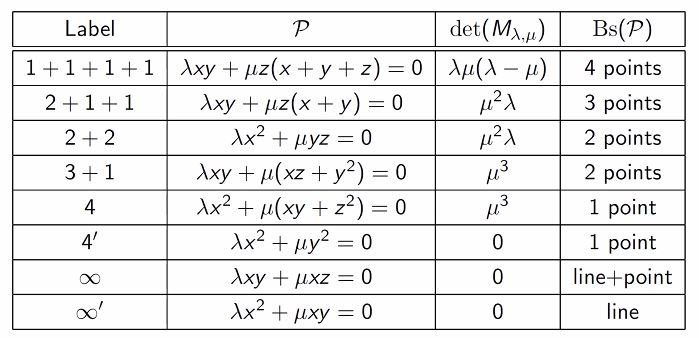
\includegraphics[width=0.4\textwidth]{./figures/L4.1}
\end{figure}

\begin{proof}[]
  \textbf{Step 1:}
  Write them down in matrix form, then just add the conics. Then the determinant is going to polynomial in $\l$, it may be a zero polynomial or its going to be a homogenous polynomial of degree 3. These three points are three reducible conics. Now choose a basis of the pencil, such that our polynomial changes.\\
  \textbf{Step 2: } the polynomial has three, two dor one root. Then we can assume,
  \begin{itemize}
    \item it's a zero polynomial
    \item It's $\l \mu (\l - \mu)$
    \item $\l \mu ^2$
    \item $\mu ^3$
  \end{itemize}
  Now to change $x, y$ and $z$. Thus we assume $f_2 = x^2$ or $f_2 = 2xy$.
  \begin{itemize}
    \item If the polynomial is not $\mu^3$, then $g_2$ is reducible
    \item If the polynomial is $\mu ^ 3$, then $g_2$ is irreducible.\\
  \end{itemize}
  \textbf{Step 3:} Take,
  $$ g_2 = 2ax^2 + bxy + 2cy^2 + dxz + eyz + eyz + 2fz^2 $$

  \begin{figure}[!ht]
  \centering
  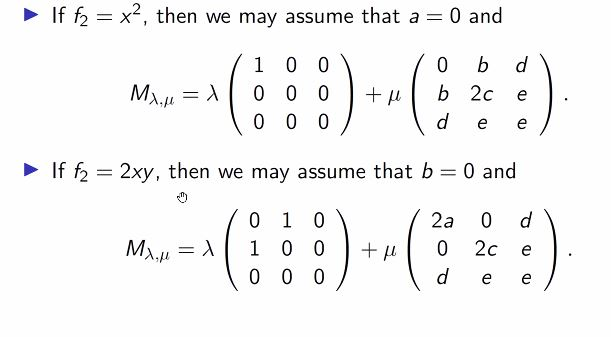
\includegraphics{./figures/L4.2}
  \end{figure}

  \textbf{Step 4:} We have $f_2 = x^2$ and
  $$ h_3 = (2bde - 2b^2f - 2cd^2)\mu^3 + (4cf - e^2)\mu^2 \l $$
  If $h_3 = 0$, pencil is reducible,
  $$ \begin{cases}
    2bde - 2b^2f - 2cd^2 = 0\\
    4cf - e^2 = 0
  \end{cases} $$
  either $c = e = b = 0$, so $g_2$ doesn't depend on $y$, or $c \ne 0$, then we can assume $c = \frac{1}{4}$, which gives $f = e^2$ and $d = 2be$, so that,
  $$ g_2 = (y + 2ez)(4bx + y + 2ez) $$
  In both cases, we can change $g_2 \in \mathcal{P}$ and coordinates so that $\mathcal{P}$ is given by,
  $$ \l x^2 + \mu y^2 = 0 $$
  similarly for $f_2 = 2xy$ and $h_3 = 0$.\footnote{This is a special case of Bertini's Theorem}
  \begin{remark}
     A pencil is 2D as nets is to 3D.
  \end{remark}

  \textbf{Step 5:} Now we assume that a cubic polynomial is not zero. So $h_3$ is $\l \mu (\l - \mu)$ or $\l \mu^2$ or $\mu^3$ and play the same game. \\
  If $f_2 = x^2$ and $\mathcal{C}$, then,
  $$ \mathcal{C} = L + L' $$
  If $L = L'$ and then $h_3 = 0$, which is impossible. Then,
  $$ L \ne L' $$
  so we can't have the lines being $x = 0$,
  \begin{itemize}
    \item $L$ is then given by $y = 0$
    \item $L'$ is given by $z = 0$
  \end{itemize}
  so that $\mathcal{P}$ is given by $\l x^2 + \mu yz = 0$\\
  \textbf{Step 6:} If $f_2 = x^2$ and $\mathcal{C}$ is irreducible then $h_3 = \mu^3$ and,
  \begin{itemize}
    \item $x= 0$ intersects with teo points
    \item $x = 0$ only intersects at some points
  \end{itemize}
  Changing coordinates we can say,
  \begin{itemize}
    \item $x = 0$ instrsects $\mathcal{C}$ by $[0 : 0 : 1]$ and $[0 : 1 :0]$.
    \item $x = 0$ is the tangent $\mathcal{C}$ at $[0 : 0 : 1]$
  \end{itemize}
  \begin{figure}[!ht]
  \centering
  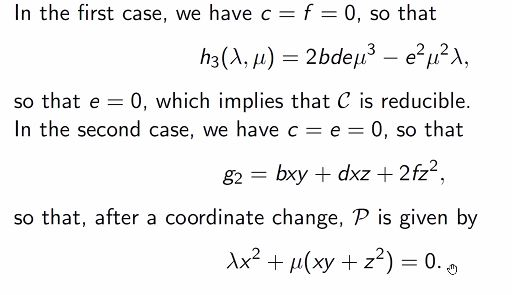
\includegraphics{./figures/L4.3}
  \end{figure}
  \textbf{Step 7: }Assume $f_2 = 2xy$ and $h_3$ is a polynomial and $g_2$ is some other polynomial. So we compute the determinant of the matrix and compare cases. \footnote{ I'm done, I'm tired.}
  Then,
  $$ \l xy + \mu (xz + y^2) = 0 $$
  \begin{ncor}
     We may assume that either $h_3 = \l\mu (\l - \mu)$ or $h_3 = \l \mu^2$
  \end{ncor}

  We conclude that $\mathcal{C}$ is reducible\\

  \textbf{Step 8:} We do some stuff relating to the fact $g_2^2 = z^2$\footnote{Typo here, I don't quite understand} and then say that $\l xy + \mu z^2 = 0$.\\
  Now we assume that the lines are distinct. So assume one of the lines don't pass through $[0 : 0 : 1]$, so map to $z = 0$ and then pencil simplifies and the fiddle for a bit.\\
  \textbf{Step 9:} Do some more cases.
\end{proof}





\end{document}
